%%%%     SETTING STARTS - DO NOT CHANGE Unless your TeX setting require so   %%
%%%%%%%%%%%%%%%%%%%%%%%%%%%%%%%%%%%%%%%%%%%%%%%%%%%%%%%%%%%%%%%%%%%%%%%%%%%%%%%
%%----------------------------------------------------------------------------------
% DO NOT Change this. It is the required setting A4 page, 11pt, onside print, book style
%%----------------------------------------------------------------------------------
\documentclass[a4paper,11pt,oneside]{book}

%%-------------------------------------
%% Page margin settings - % half inch margin all sides (recommended)
%%-------------------------------------
\usepackage[margin=1.2in]{geometry} 

%%-------------------------------------
%% Font settings - % CM San or Ariel (recommended)
%%-------------------------------------
% Switch the following two line off: to revert back to default LaTex font (NOT recommended)
\usepackage{amsfonts}
\renewcommand*\familydefault{\sfdefault}

%%-------------------------------------
%% Math/Definition/Theorem/Algorithm packages settings 
%%-------------------------------------
\usepackage[cmex10]{amsmath}
\usepackage{amssymb}
\usepackage{amsthm}
\usepackage{fancyhdr}
\usepackage{amsmath}
\usepackage{lmodern}
\newtheorem{mydef}{Definition}
\newtheorem{mytherm}{Theorem}
%%-------------------------------------
%% Algorithms/Code Listing environment settings  - 
%% Please do not change these settings
%%-------------------------------------
\usepackage{algorithm}
\usepackage{algpseudocode}
\renewcommand{\algorithmicrequire}{\textbf{Input:}}
\renewcommand{\algorithmicensure}{\textbf{Output:}}
\usepackage[utf8]{inputenc}
\usepackage{listings}
\usepackage{xcolor}
\definecolor{codegreen}{rgb}{0,0.6,0.1}
\definecolor{codegray}{rgb}{0.5,0.5,0.5}
\definecolor{codeblue}{rgb}{0.10,0.00,1.00}
\definecolor{codepurple}{rgb}{0.58,0,0.82}
\definecolor{backcolour}{rgb}{1.0,1.0,1.0}

\lstdefinestyle{mystyle}{
    backgroundcolor=\color{backcolour},   
    commentstyle=\color{codegreen},
    keywordstyle=\color{codeblue},
    numberstyle=\tiny\color{codegray},
    stringstyle=\color{codepurple},
    basicstyle=\ttfamily\footnotesize,
    breakatwhitespace=false,         
    breaklines=true,                 
    captionpos=b,                        
    keepspaces=true,                 
    numbers=left,                    
    numbersep=5pt,                  
    showspaces=false,                
    showstringspaces=false,
    showtabs=false,                  
    tabsize=2,
    frame=none
}
\lstset{style=mystyle}

%%-------------------------------------
%% Graphics/Figures environment settings
%%-------------------------------------
\usepackage{graphicx}
\usepackage{subfigure}
\usepackage{caption}
\usepackage{lipsum}

%%-------------------------------------
%% Table environment settings
%%-------------------------------------
\usepackage{multirow}
\usepackage{rotating}
\usepackage{makecell}
\usepackage{booktabs}
%\usepackage{longtable,booktabs}

%%-------------------------------------
%% List of Abbreviations settings
%%-------------------------------------
\usepackage{enumitem}
\newlist{abbrv}{itemize}{1}
\setlist[abbrv,1]{label=,labelwidth=1in,align=parleft,itemsep=0.1\baselineskip,leftmargin=!}

%%-------------------------------------
%% Bibliography/References settings   - Harvard Style was used in this report
%%-------------------------------------
\usepackage[hidelinks]{hyperref}
\usepackage[comma,authoryear]{natbib}
\renewcommand{\bibname}{References} % DO NOT remove or switch of 

%%-------------------------------------
%% Appendix settings     
%%-------------------------------------
\usepackage[toc]{appendix}
%%%%%%%%%%%%%%%%%%%%%%%%%%%%%%%%%%%%%%%%%%%%%%%%%%%%%%%%%%%%%%%%%%%%%%%%%%%%%%%%%%%%%%%
%%%%                     SETTING ENDS                                            %%%%%%
%%%%%%%%%%%%%%%%%%%%%%%%%%%%%%%%%%%%%%%%%%%%%%%%%%%%%%%%%%%%%%%%%%%%%%%%%%%%%%%%%%%%%%%


\fancyhf{}
\fancyhead[L]{EE4033-Algorithms Spring 2023}
\fancyhead[R]{Steven Wong, T11705207}
\renewcommand\headrulewidth{0pt}
\pagestyle{fancy}

\begin{document}
\noindent\makebox[\textwidth][c]{\Large\bfseries Homework Assignment 2 (No Collaborators)}
\normalsize

% Question 1
\begin{enumerate}
  \item {\textbf{Exercise 6.5$-$8}} 
  \begin{algorithm}
    \caption{Heap-Delete Algorithm}
    \begin{algorithmic}[1]
        \Function{Heap-Delete}{$\mathbf{A, i}$}
        \State{$A[i] \gets A[n]$} % Replace the deleted node with the last node
        \State{$n \gets n-1$} % Decrease the heap size by 1
        \State{$HEAPIFY(A, i)$} % Maintain the max-heap property
        \EndFunction
    \end{algorithmic}
\end{algorithm}

  % Question 2
  \item {\textbf{Exercise 7.2$-$3}}
  The worst case running time of Quicksort is $\Theta\left(n^2\right)$ for a descending order array when the slection of the pivot is always the right element. 
  In this case, each iteration of Partition reduces the size of the sub-array by 1. Thus, we have a recurrence relation equal to 
  \[T(n-1)+\Theta(n) = \Theta(n^2)\]

  % Question 3
  \item {\textbf{Modified Exercise 8.2$-$1}} First I tranposed the alphabetical characters to numbers giving me the following values:
  $$ 14-20-21-5-5-3-19-1-12-7-15-18-9-20-8-13$$

  Then I used the counting sort algorithm to sort the array with indices from 0-25 representing each alphabetical value. The result is:
  $$ 1-0-1-0-2-0-1-1-1-0-0-1-1-1-1-0-0-1-1-2-1-0-0-0-0-0$$

  Forming the next index array, I obtained the following result by adding the previous index to the current index:
  $$ 1-1-2-2-4-4-5-6-7-7-7-8-9-10-11-11-11-12-13-15-16-16-16-16-16-16$$

  Finally, I used the index array to sort the original array into the following result:
  $$ A-C-E_1-E-2-G-H-I-L-M-N-O-P-R-S-T_1-T_2-U$$
  
  % Question 4
  \item {\textbf{Exercise 8.2$-$4}} Given $n$ integers in the range of 0 to $k$ as array $A$, create an $k$ sized auxiliary array $B$ initialized to $0$.
  For each element $i \text{ in} A$ increment $B[A[i]]$. Compute the running sum for each element $i$ in $B$ 
  and obtain the number of elements less than or equal to $i$. At this point, this is the initial steps in counting sort.
  To compute the number of elements in range $[a..b]$ we now have an $\Theta(1)$ computation: $B[b] - B[a]$
  in range $[a..b]$   
  
  % Question 5
  \item {\textbf{Exercise 9.3$-$7}} With the assumption that the set S is a sorted array of elements, we have the median given by
  index $n/2$. Then the closest $k$ elements must be within the range of $(n-k)/2 \le n/2 \le (n+k)/2$. We can use linear search 
  to traverse through these indices to find elements greater than $(n-k)/2$, not equal to $n/2$, and less than $(n+k)/2$.
  
  % Question 6
  \item {\textbf{Search Trees}}
  \begin{figure}[h]
    \centering
    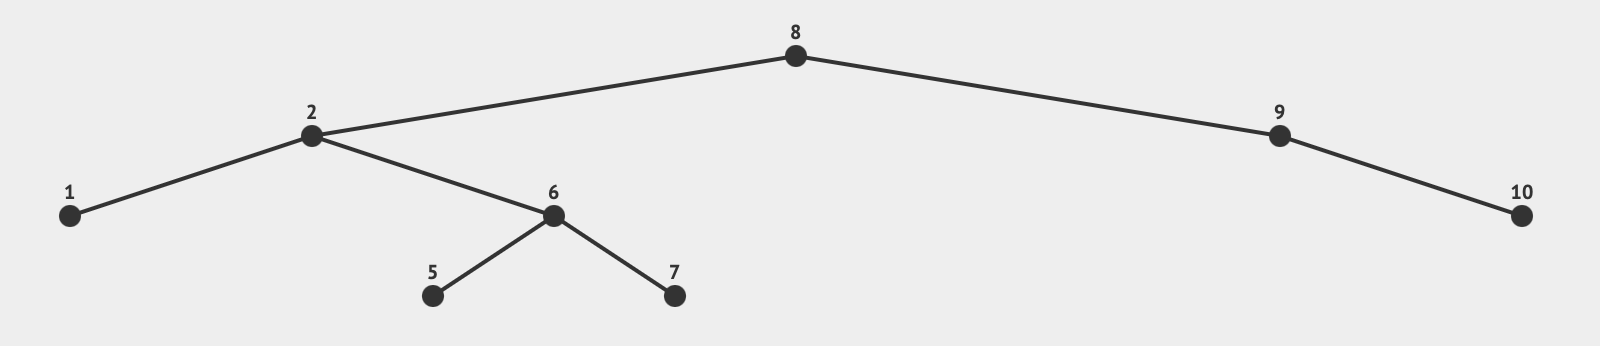
\includegraphics[width=0.8\textwidth]{6a.png}
    \caption{Binary Search Tree}\label{fig:6a}
  \end{figure}
  \begin{figure}[h]
    \centering
    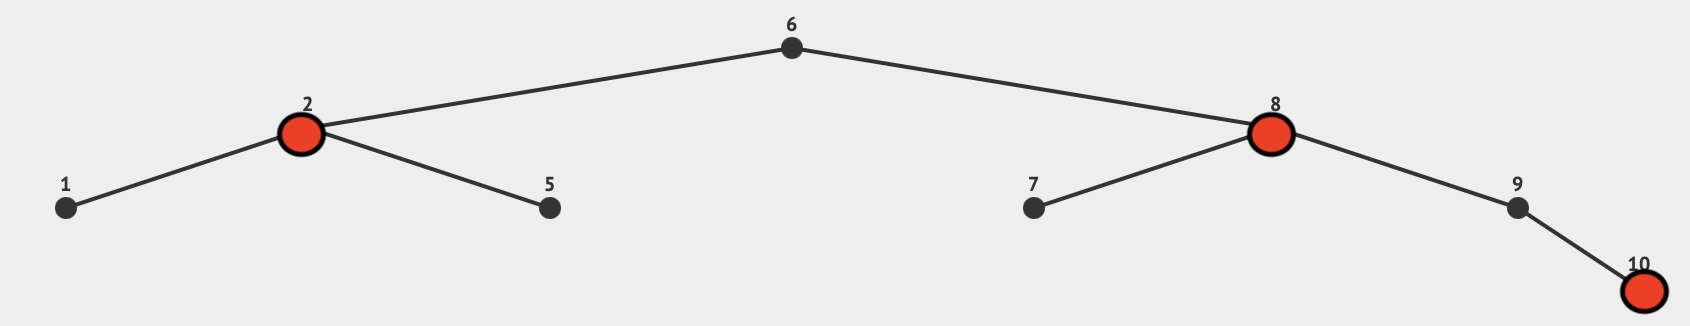
\includegraphics[width=0.8\textwidth]{6b.png}
    \caption{Red Black Tree}\label{fig:6b}
  \end{figure}
  \begin{figure}
    \centering
    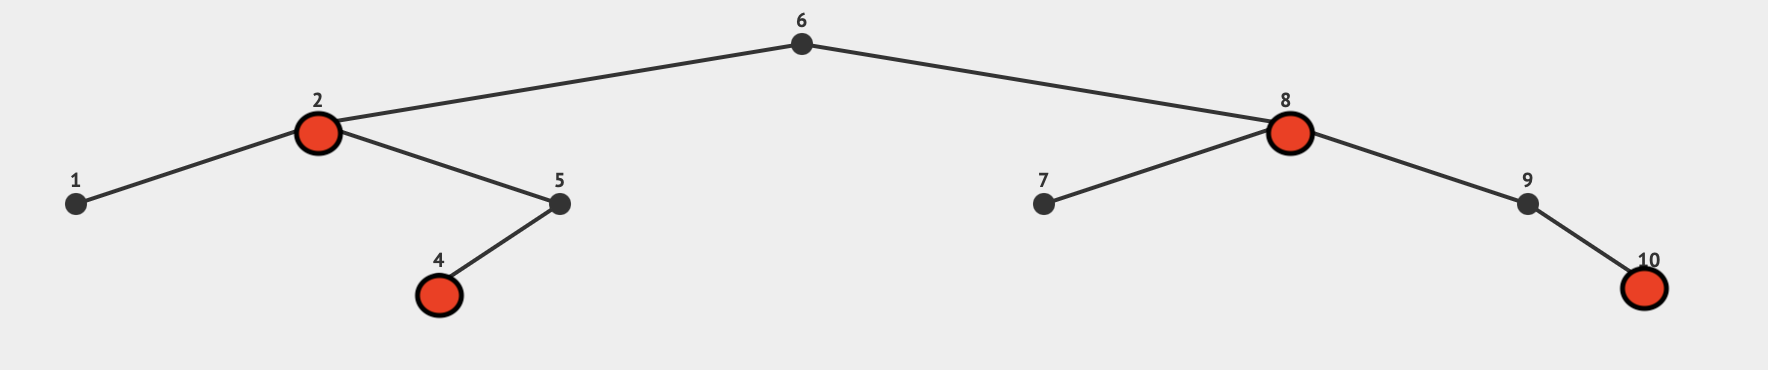
\includegraphics[width=0.8\textwidth]{6c.png}
    \caption{Red Black Tree Add 4}\label{fig:6c}
  \end{figure}
  \begin{figure}
    \centering
    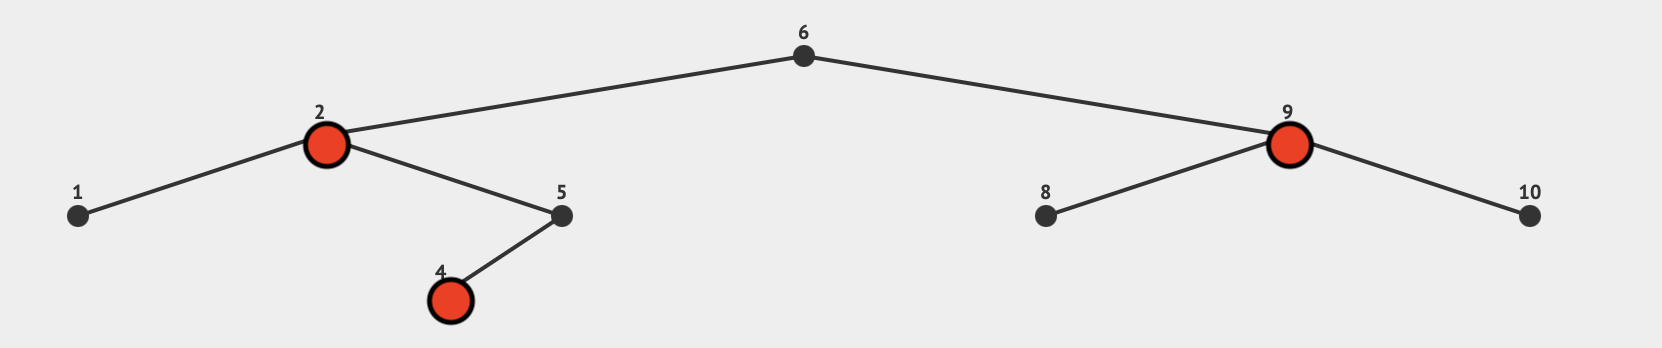
\includegraphics[width=0.8\textwidth]{6d.png}
    \caption{Red Black Tree Remove 7}\label{fig:6d}
  \end{figure}
  
  % Question 7
  \item {\textbf{Dynamic Programming Implementations}}
  \\ a. Find an optimal parenthesization to a matrix-chain product whose sequence of dimensions is < 3, 5, 7, 9, 11 >.
  \\ b. Determine an LCS of < C, A, B, A, C, B, D > and < A, D, B, A, C, D >.
  \\ c. Determine the cost and structure of an optimal binary search tree for a set of $n=6$ keys with the following probabilities: $p_i=0.05,0.09,0.10,0.05,0.12,0.15, i=1, . ., 6$, respectively, and $q_i=$ $0.03,0.06,0.07,0.11,0.08,0.05,0.04, i=0, \ldots, 6$, respectively
  
  % Question 8
  \item {\textbf{(20 pts) Given a log of wood of length $k$, Woody the woodcutter will cut it once, in any place you choose, for the price of $k$ dollars. Suppose you have a log of length $L$, marked to be cut in $n$ different locations labeled $1,2, \ldots, n$. For simplicity, let indices 0 and $n+1$ denote the left and right endpoints of the original log of length $L$. Let the distance of mark $i$ from the left end of the log be $d_i$, and assume that $0=d_0<d_1<d_2<\ldots<d_n<d_{n+1}=L$. The wood-cutting problem is the problem of determining the sequence of cuts to the $\log$ that will (1) cut the log at all the marked places, and (2) minimize your total payment to Woody.}}
  \\ a. (4 pts) Give an example with $L=4$ illustrating that two different sequences of cuts to the same marked log can result in two different costs.
  \\ b. (9 pts) Let $c(i, j)$ be the minimum cost of cutting a log with left endpoint $i$ and right endpoint $j$ at all its marked locations. Suppose the log is cut at position $m$, somewhere between $i$ and $j$. Define the recurrence of $c(i, j)$ in terms of $i, m, j, d_i$, and $d_j$. Briefly justify your answer.
  \\ c. (7 pts) Using part (b), give an efficient algorithm to solve the wood-cutting problem. Use a table $C$ of size $(n+1) \times(n+1)$ to hold the values $C[i][j]=c(i, j)$. What is the running time of your algorithm?
  
  % Question 9
  \item {\textbf{(20 pts) Let $X=x_1 x_2 \ldots x_m$ and $Y=y_1 y_2 \ldots y_n$ be two character strings. This problem asks you to find the maximum common substring length for $X$ and $Y$. Notice that substrings are required to be contiguous in the original strings. For example, photograph and tomography have common substrings $p h$, to, ograph, etc. The maximum common substring length is 6 .}}
  \\ a. (a) (4 pts) The following gives the computation of the maximum common suffix and substring lengths on the two strings, $A B A B$ and $B A B$, similar to the table used for computing the length of LCS in class. Only partial results are given. Please complete all the entries in the table.

\end{enumerate}
\end{document}